%# -*- coding: utf-8-unix -*-
\chapter{多端口构造符号化约简方法探索}
\label{chap:mp}

本章对多端口电路的构造进行探索,由于期望将来能希望针对多端口情况下的模拟电路模型降阶方法提供基础。

\section{共模抑制比与电源抑制比介绍}

运算放大器除了差分增益响应以及相对应的相位变化,别的设计指标也是极为关键的。
在近几年兴起的生物电路中,由于生物电信号的较为微弱的特性,共模及电源噪声信号的影响对相关的运算放大器设计工作提出了很高的要求\parencite{Sawan-CMRR-1999,Abdullah-Biopotential-2015,Paul-22dBPSRR-2012}。
目前对这两方面指标的自动化辅助工具的研究比较欠缺,故十分需要有相应的工具对此种类型的电路分析工作进行指导与辅助。

根据\parencite{GRAY-Analog}中的定义,可根据图\ref{fig:cmps}中的示意给出共模抑制比(Common Mode Rejection Ratio, $CMRR$)和电源抑制比(Power Supply Rejection Ratio, $PSRR$)的定义。

\begin{figure}[!htp]
	\centering
	\includegraphics[width=0.8\textwidth]{chap4/CMPS.eps}
	\bicaption[fig:cmps]{共模抑制比及电源抑制比定义}{共模抑制比及电源抑制比定义}{Fig}{CMRR and PSRR definition}
\end{figure}

首先给出CMRR的定义,如图\ref{fig:cmps}左侧所示,一个差分运算放大器有两个差分输入端,如果在两个输入端输入叠加在共模信号上的差分信号。
用$v_d$和$v_{cm}$代表信号的差模和共模部分,那么我们可以得到运放的输出信号的差模部分有$v_{out}^{d} = A_v v_d$;而共模输出信号有$v_{out}^{cm} = A_{cm} v_{cm}$。
这里$A_v$和$A_{cm}$代表了运放的差模和共模增益。那么可以将CMRR定义为差模增益与共模增益的比值,如下式所示。

\begin{equation}
CMRR = \left|\frac{A_v}{A_{cm}}\right|
\end{equation}

接着给出PSRR的定义,如图\ref{fig:cmps}右侧所示,运放的电源电压部分给上一个小信号激励$v_{dd}$。
那么运放输出中由电源处提供的信号可以表示为$v_{out}^{ps} = A_{ps}v_{dd}$,这里$A_{ps}$代表了运放的电源增益。
故可以将PSRR定义为差模增益与电源增益的比值,如下式所示。

\begin{equation}
PSRR = \left|\frac{A_v}{A_{ps}}\right|
\end{equation}

可以看到运放的CMRR和PSRR均是通过小信号计算得到,故可以使用符号化分析得到相应的结果。
同时可以看到在分析CMRR和PSRR的过程中用到3个增益:$A_v$、$A_{cm}$和$A_{ps}$。
这三者的输出端均为测量电压,且为同一个端口的测量,故满足上一节所给出的定理\ref{thm:mpcon},那么可以使用单根的GPDD多端口的符号化分析方法对CMRR和PSRR进行分析。

\section{CMRR和PSRR在多端口构造下的计算方法}

CMRR和PSRR的分析总共涉及3个输入输出对:

\begin{enumerate}
	\item 差分输入到输出端的差模电压增益$A_v$
	\item 共模噪声到输出端的共模电压增益$A_{cm}$
	\item 电源扰动到输出端的电源电压增益$A_{ps}$
\end{enumerate}

这三组输入输出对对应了不同的输入信号端口。
因此在符号化构建的过程中,我们只需要在输入网表顶部给出3组VCVS的受控源,即可完成符号化网表的构建。
这三组受控源这里分别用$X_v$、$X_{cm}$和$X_{ps}$三个符号给出,经过多端口符号化构造过程,可以得到类似于图\ref{fig:cmpsgpdd}的GPDD结构。

\begin{figure}[!htp]
	\centering
	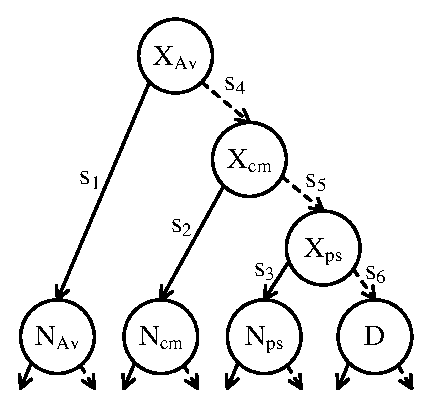
\includegraphics[width=0.35\textwidth]{chap4/CMPSGPDD.eps}
	\bicaption[fig:cmpsgpdd]{多端口方法构造CMRR及PSRR的GPDD结构}{多端口方法构造CMRR及PSRR的GPDD结构}{Fig}{GPDD Structure for multi-port construction of CMRR and PSRR}
\end{figure}

这里的子GPDD结构由$N_{Av}$,$N_{cm}$,$N_{ps}$和$D$这四个GPDD节点为根组成。
我们将使用他们的符号化结果来计算得到CMRR和PSRR的值。
那么根据GPDD的求值规则,辅以符号化电路元件约减的性质,可以得到之前的三个增益可用下式计算得到。

\begin{eqnarray}
A_v     &= \frac{1}{X_{Av}} &= - s_1 s_4 s_5 s_6 \frac{f\left(N_{Av}\right)}{f\left(D\right)}\\
A_{cm}  &= \frac{1}{X_{cm}} &= - s_2 s_5 s_6 \frac{f\left(N_{cm}\right)}{f\left(D\right)}\\
A_{ps}  &= \frac{1}{X_{ps}} &= - s_3 s_6 \frac{f\left(N_{ps}\right)}{f\left(D\right)}
\end{eqnarray}

同时,根据CMRR和PSRR的定义,可以简化CMRR和PSRR在GPDD中的计算如下:

\begin{eqnarray}
CMRR &=& s_1 s_2 s_4 \frac{f\left(N_{Av}\right)}{f\left(N_{cm}\right)}\\
PSRR &=& s_1 s_3 s_4 s_5 \frac{f\left(N_{Av}\right)}{f\left(N_{ps}\right)}
\end{eqnarray}

值得注意的是,这里GPDD的构造过程只需要一次。
只要知道所有电路符号元件的值,而后$A_v$,$CMRR$和$PSRR$的数值结果可以通过自底向上遍历GPDD结构同时得到,节省了计算时间。
这样的计算效率在之前提出的一些符号化方法中是不可行的\parencite{Gielen-ISAAC-1989}。

根据第\ref{chap:gpddtheory}章中介绍的敏感度计算方法,通过简单的推导即可知道,CMRR和PSRR的敏感度也可以通过如下的计算得到:

\begin{equation}
Sens\left( {{CMRR},{W_i}} \right) = Sens\left( {{A_{v}},{W_i}} \right) - Sens\left( {{A_{cm}},{W_i}} \right)
\end{equation}

\begin{equation}
Sens\left( {{PSRR},{W_i}} \right) = Sens\left( {{A_{v}},{W_i}} \right) - Sens\left( {{A_{ps}},{W_i}} \right)
\end{equation}

这意味着我们需要求得三个增益的敏感度,即可得到CMRR和PSRR的敏感度。
同时,由于所有的计算均在同一个GPDD上进行,所以可以高效地求得相应的结果。

\section{共模抑制比与电源抑制比测试结果}

\subsection{多端口构造方法的双图决策树的时间空间复杂度比较}

这里的测试电路选用了图\ref{fig:two_stage}和图\ref{fig:folded_cascode}中的折叠共源共栅运放和两级运放结构。

\begin{figure}[!htp]
	\centering
	\includegraphics[width=0.7\textwidth]{chap4/res/TSRes.eps}
	\bicaption[fig:trres]{两级运放的$CMRR$及$PSRR$的频率响应结果}{两级运放的$CMRR$及$PSRR$的频率响应结果}{Fig}{Frequency response for $CMRR$ and $PSRR$ in two-stage opamp}
\end{figure}

\begin{figure}[!htp]
	\centering
	\includegraphics[width=0.7\textwidth]{chap4/res/FDRes.eps}
	\bicaption[fig:fcres]{折叠共源共栅运放的$CMRR$及$PSRR$的频率响应结果}{折叠共源共栅运放的$CMRR$及$PSRR$的频率响应结果}{Fig}{Frequency response for $CMRR$ and $PSRR$ in folded-cascode opamp}
\end{figure}

相应的小信号电路元件参数通过HSPICE的数值仿真结果得到,并构建相应的GPDD结构。
计算得到的CMRR和PSRR的频率响应曲线在图\ref{fig:trres}和图\ref{fig:fcres}中展示。
可以看到仿真结构与HSPICE的数值结果十分吻合,所以GPDD符号化计算的结果是有效的。

\begin{table}[!htp]
	\bicaption[tab:tscmpsgpdd]{两级运放的单独构造与多端口构造的时空性能比较}{两级运放的单独构造与多端口构造的时空性能比较}{Table}{Comparison between separated and multi-port constructions for the two-stage opamp}
	\centering
	\begin{tabular}{*{3}{c}}
		\hline
		       情况         & $|\mbox{GPDD}|$ & 构造时间 ($\mu s$) \\ \hline
		 单独构造$A_v$的GPDD   &      2251       &     522.0      \\
		单独构造$A_{cm}$的GPDD &      2615       &     408.7      \\
		单独构造$A_{ps}$的GPDD &      3933       &     632.0      \\
		       总计         &      8799       &     1562.7     \\ \hline
		    多端口构造GPDD     &      4871       &     730.1      \\ \hline
		      改进程度        &     44.6\%      &      2.1x      \\ \hline
	\end{tabular}
\end{table}

\begin{table}[!htp]
	\bicaption[tab:fccmpsgpdd]{折叠共源共栅运放的单独构造与多端口构造的时空性能比较}{两级运放的单独构造与多端口构造的时空性能比较}{Table}{Comparison between separated and multi-port constructions for the folded-cascode opamp}
	\centering
	\begin{tabular}{*{3}{c}}
		\hline
		       情况         & $|\mbox{GPDD}|$ & 构造时间 ($s$) \\ \hline
		 单独构造$A_v$的GPDD   &      24228      &   155.2    \\
		单独构造$A_{cm}$的GPDD &      25706      &   122.0    \\
		单独构造$A_{ps}$的GPDD &      32918      &   173.6    \\
		       总计         &      82852      &   450.8    \\ \hline
		    多端口构造GPDD     &      35424      &    78.7    \\ \hline
		      改进程度        &     57.2\%      &    5.7x    \\ \hline
	\end{tabular}
\end{table}

我们也统计我们的软件实现性能来证明多端口构造得到的GPDD共享结果的优势。
首先,我们针对三种增益$A_v$,$A_{cm}$和$A_{ps}$分别单独构造GPDD结构,并统计相应的构造时间和GPDD节点个数。
其相应的结果在表\ref{tab:tscmpsgpdd}和表\ref{tab:fccmpsgpdd}中展现。
总计一栏将上述三个增益分别的表现进行了求和,反映分别构造总复杂度。
然后采用多端口方式构造同时对三个增益构造GPDD。
从表中的数据可以明显地看到多端口电路构造方式的优势,利用更少的时间和更少的计算空间完成了整体的计算。

\if@0
\subsubsection{两级运放的电路的参数扫描结果}

由于符号化一次构造,多次计算的优良性质,符号化计算可以快速地对电路的参数进行扫描,并从中观察电路元件取值对电路性能的影响。
这里我们对两级运放的补偿部分的两个电路元件补偿电容$C_c$和调零电阻$R_z$进行参数扫描,以观察CMRR和PSRR与其之间的关系。

\begin{figure}[!htp]
	\centering
	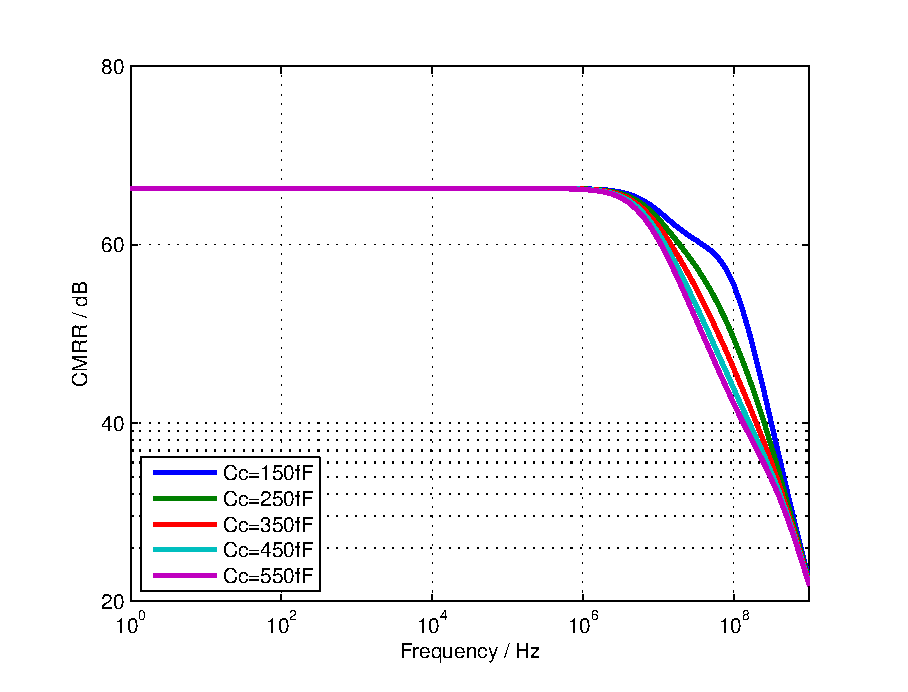
\includegraphics[width=0.7\textwidth]{chap4/res/CMRR_CC.eps}
	\bicaption[fig:cmrrcc]{两级运放针的$CMRR$对补偿电容$C_c$的参数扫描结果}{两级运放针的$CMRR$对补偿电容$C_c$的参数扫描结果}{Fig}{Parameter sweep results for $CMRR$ of compensation capacitor $C_c$ in two-stage opamp}
\end{figure}

\begin{figure}[!htp]
	\centering
	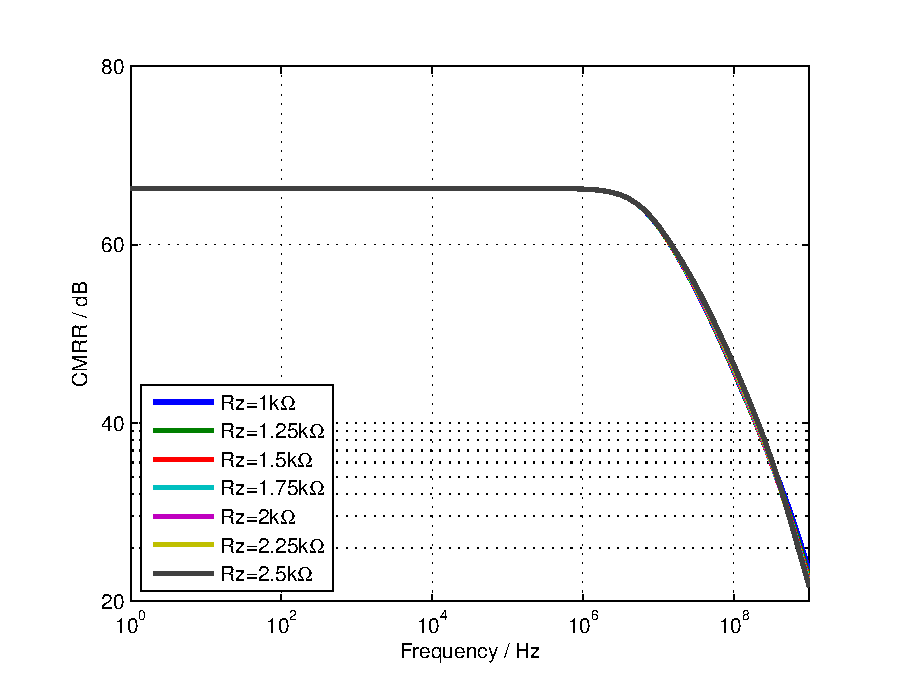
\includegraphics[width=0.7\textwidth]{chap4/res/CMRR_Rz.eps}
	\bicaption[fig:cmrrrz]{两级运放针的$PSRR$对调零电阻$R_z$的参数扫描结果}{两级运放针的$CMRR$对补偿电容$R_z$的参数扫描结果}{Fig}{Parameter sweep results for $CMRR$ of compensation capacitor $R_z$ in two-stage opamp}
\end{figure}

\begin{figure}[!htp]
	\centering
	\includegraphics[width=0.7\textwidth]{chap4/res/PSRR_CC.eps}
	\bicaption[fig:psrrcc]{两级运放针的$PSRR$对补偿电容$C_c$的参数扫描结果}{两级运放针的$PSRR$对补偿电容$C_c$的参数扫描结果}{Fig}{Parameter sweep results for $PSRR$ of compensation capacitor $C_c$ in two-stage opamp}
\end{figure}

\begin{figure}[!htp]
	\centering
	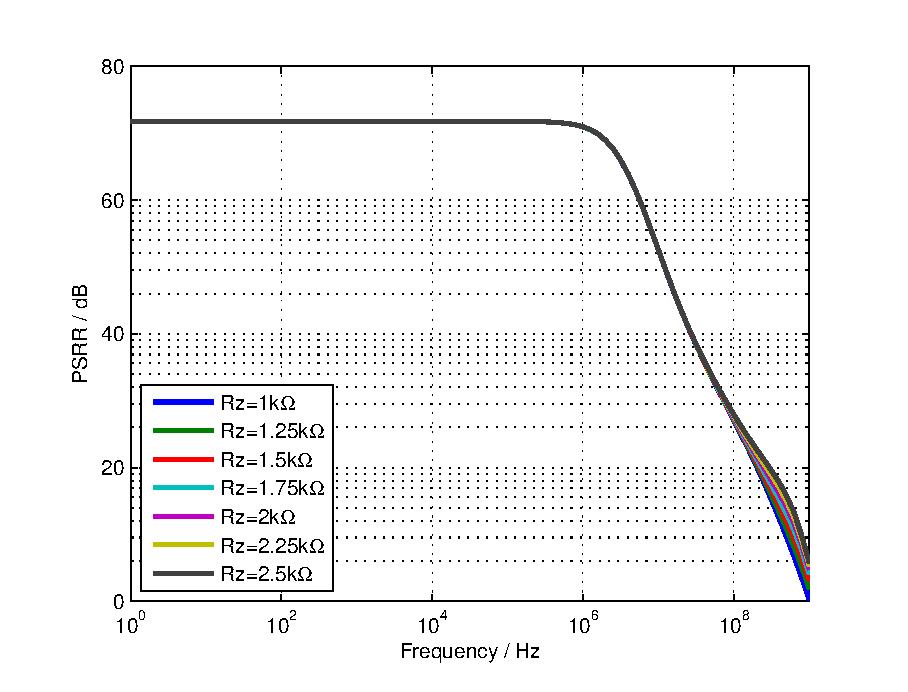
\includegraphics[width=0.7\textwidth]{chap4/res/PSRR_Rz.eps}
	\bicaption[fig:psrrrz]{两级运放针的$PSRR$对调零电阻$R_z$的参数扫描结果}{两级运放针的$PSRR$对补偿电容$R_z$的参数扫描结果}{Fig}{Parameter sweep results for $PSRR$ of compensation capacitor $R_z$ in two-stage opamp}
\end{figure}

根据图\ref{fig:cmrrcc}至图\ref{fig:psrrrz}的结果,可以看到CMRR和PSRR在高频接近转角频率处对于补偿电容$C_c$的变化较为敏感;
然而在同样的区域调零电阻的影响相对小了很多。
根据这些信息,电路工程师可以更方便地观察不同元件取值的影响,从而更有效率地进行电路设计。

\fi

\subsection{敏感度方法进行电路参数优化共模电源抑制比}

最后,我们对CMRR和PSRR的敏感度进行计算,并尝试通过敏感度进行电路优化。
这里仍然针对两级运放进行分析,我们对其中的第一级和第二级的输入MOS管$M_1$和$M_6$的尺寸求取敏感度。
相应的敏感度结果在图\ref{fig:SensW6}和图\ref{fig:SensW6}中展现。

\begin{figure}[!htp]
	\centering
	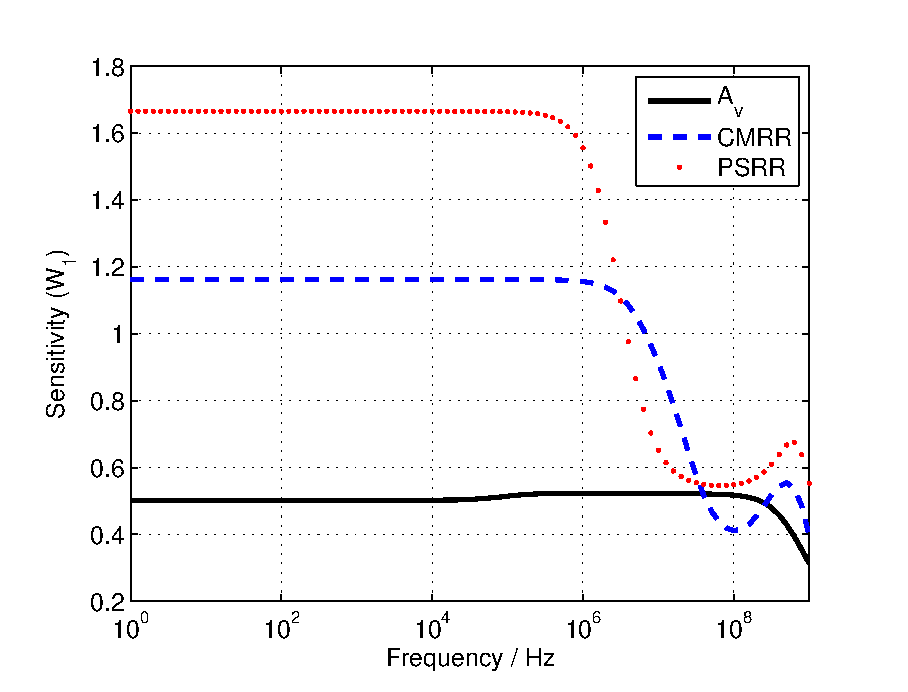
\includegraphics[width=0.7\textwidth]{chap4/res/SensW1.eps}
	\bicaption[fig:SensW1]{两级运放针对$W_1$的敏感度分析结果}{两级运放针对$W_1$的敏感度分析结果}{Fig}{Sensitivity results of $W_1$ in two-stage opamp}
\end{figure}

\begin{figure}[!htp]
	\centering
	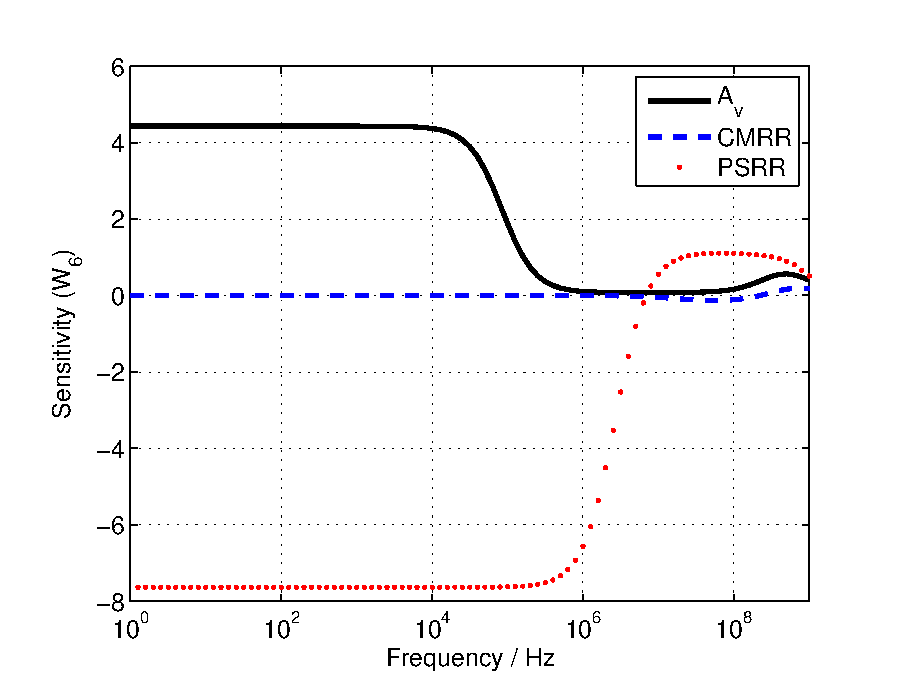
\includegraphics[width=0.7\textwidth]{chap4/res/SensW6.eps}
	\bicaption[fig:SensW6]{两级运放针对$W_6$的敏感度分析结果}{两级运放针对$W_6$的敏感度分析结果}{Fig}{Sensitivity results of $W_6$ in two-stage opamp}
\end{figure}

根据图中所展现的结果,我们看到$W_1$与三种电路指标$A_v$、$CMRR$和$PSRR$均正相关,故增大$W_1$将同时增大三种性能指标。
然而$W_6$情况则不同,如增大$W_6$的话,差分增益$A_v$会有所提升,$CMRR$基本保持不变,而$PSRR$则会下降。

我们在实际对运放进行了尺寸优化($W_1$从原有的$20\mu m$变为$30\mu m$,$W_6$从原有的$30\mu m$变为$31\mu m$)后,将相应的数据变化记录于表\ref{tab:sensw1}和表\ref{tab:sensw6}中。

\begin{table}[!htp]
	\bicaption[tab:sensw1]{$W_1$的DC敏感度分析结果及优化}{$W_1$的DC敏感度分析结果及优化}{Table}{Sensitivity analysis at DC of $W_1$}
	\centering
	\begin{tabular}{c|c|c|c|c|c}
		\hline
		\multirow{2}{*}{指标} & \multicolumn{2}{c|}{$W_1=20\mu m$} & \multicolumn{2}{c|}{$W_1=30\mu m$} & \multirow{2}{*}{比率} \\ \cline{2-5}
		                    &       值        &        敏感度        &       值        &        敏感度        &  \\ \hline
		       $A_v$        & 2.84K (69.1dB) &       0.502       & 3.41K (70.7dB) &       0.401       &  +20.0\% (+1.6dB)   \\ \hline
		      $CMRR$        & 2.07K (66.3dB) &       1.162       & 3.05K (69.7dB) &       0.802       &  +47.3\% (+3.4dB)   \\ \hline
		      $PSRR$        & 3.87K (71.8dB) &       1.665       & 6.92K (76.8dB) &       1.237       &  +78.8\% (+5.0dB)   \\ \hline
	\end{tabular}
\end{table}

\begin{table}[!htp]
	\bicaption[tab:sensw6]{$W_6$的DC敏感度分析结果及优化}{$W_6$的DC敏感度分析结果及优化}{Table}{Sensitivity analysis at DC of $W_6$}
	\centering
	\begin{tabular}{c|c|c|c|c|c}
		\hline
		\multirow{2}{*}{指标} & \multicolumn{2}{c|}{$W_6=30\mu m$} & \multicolumn{2}{c|}{$W_6=31\mu m$} & \multirow{2}{*}{比率} \\ \cline{2-5}
		                    &       值        &        敏感度        &       值        &        敏感度        &  \\ \hline
		       $A_v$        & 2.84K (69.1dB) &       4.43        & 3.04K (69.7dB) &       -0.20       &  +7.04\% (+0.6dB)   \\ \hline
		      $CMRR$        & 2.07K (66.3dB) &      6.1e-8       & 2.07K (66.3dB) &      9.4e-8       &     +0\% (+0dB)     \\ \hline
		      $PSRR$        & 3.87K (71.8dB) &       -7.63       & 3.32K (70.4dB) &       -2.83       &  -14.2\% (-1.4dB)   \\ \hline
	\end{tabular}
\end{table}

可以看到在尺寸调整后,三种电路指标$A_v$、$CMRR$和$PSRR$均按预期发生了变化。
同时由于敏感度的定义,即可知道电路性能变化比率与敏感度基本成正比,这在表中的数据也得到了相应的验证。
高敏感度带来了更快的性能增长。
另外,还应观察到在电路尺寸改变后电路的敏感度也发生了变化。
例如,表\ref{tab:sensw6}中的有关$A_v$的敏感度已经由正值变为了负值,说明继续增大$W_6$将对电路的增益带来不好的效果。

\section{本章小结}

本章尝试了对一种用于CMRR和PSRR的计算的符号化多端口电路构造计算方法进行了探索,以期望用于将来的针对CMRR和PSRR的电路简化方法。
首先,介绍了$CMRR$和$PSRR$的基本概念与相应的计算流程,并利用敏感度分析方法对现有电路进行调整优化。
最后,通过算法的时间空间的复杂度,验证了GPDD构造的高效性,并用敏感性分析辅助电路优化等测试证明了这种构造方法的有效性。